\svnidlong
{$HeadURL$}
{$LastChangedDate$}
{$LastChangedRevision$}
{$LastChangedBy$}
\framebox{Author: \svnauthor|Rev: \svnrev|Last change: \svndate}% - URL: \url{\svnkw{HeadURL}}}
\section{Introduction}
Synchrotron radiation based x-ray tomographic microscopy (SRXTM) is a powerful method for the non-destructive three-dimensional imaging of a broad kind of materials with a resolution on the micrometer scale.

At TOMCAT -- the beamline for TOmographic Microscopy and Coherent rAdiology experimenTs~\cite{Stampanoni2007} at the Swiss Light Source at the Paul Scherrer Institute in Villigen, Switzerland -- more than 20 user groups are presently working in very different research areas, ranging from biology, medicine and palaeontology to materials science, geology and process engineering. SRXTM enables the user to have a qualitative and quantitative measurement and analysis of nearly any structure.

\subsection{Background}
Various applications depend on the availability of high resolution tomographic images of the studied sample. The available field of view (FOV) of microscopy based imaging methods like synchrotron based tomographic beam lines and micro-computed tomography stations is limited by the camera and microscope optics. To be able to obtain images with a broad FOV one has to use lower magnifications to cover bigger samples. 
To record tomographic datasets at TOMCAT with a resolution of around \unit{1}{\micro\meter}, the sample diameter has to be smaller than \unit{1}{\milli\meter}. This constraint can be overcome with so called local tomography, where the sample diameter is bigger than the FOV, but this a) introduces image artifacts at the edges of the reconstructed slices and b) does not solve the need for a bigger FOV many users share.

\subsection{Enhancing the Field of View}
An increase of the FOV parallel to the rotation axis of the sample can be achieved through the stacking of multiple scans on top of each other. This stacking has been achieved at TOMCAT through accurately controlling the end-station setup and sample position.
This means that the final reconstructions can simply be stacked on top of each other, even if they have been acquired in different scans. For this imaging mode, the scanning time linearly increases with the sample size.

Generally, to be able to accurately reconstruct a sample, we have to fulfill the sampling theorem for computed tomography. \citet{Cormack1978} stated, that for a sample of the size $k$ (in beam diameter units) the number of independent pieces of information obtainable is exactly\todo{better equation? or should we cite~\cite{Kak2002}, where $N$ pixels $=N$ proj.?}
\begin{equation}
n(k+\frac{1}{2})%\text{ where }n=\text{ NumProj and }k=\text{Object-Diameter in beam diameter units}
\end{equation}

If we thus aim to enlarge the FOV of the tomographic images perpendicular to the rotation axis of the sample, it is not only necessary to stitch together several projection images, but also it is necessary to record a bigger amount of projections in the lateral parts of the sample compared to the central parts of the sample to be able to fulfill the sampling theorem. This leads to a increase in imaging and post-processing time as compared to a standard scan with a comparably smaller FOV. Let us assume that we have a sample that could be imaged using three overlapping FOVs of \unit{\numprint{1024}}{pixels}, we have to obtain at least \unit{\numprint{3072}}{projections} in the lateral parts of the sample to fulfill the aforementioned sampling theorem.\todo{explain in depth $>$ materials \& methods?}\todo{explain overlap $>$ materials \& methods?}

Figure~\ref{fig:overlapping scans} depicts the details of the overlapping scans.

\begin{figure}[tb]
	\centering
		
\includegraphics[width=\imsize]{img/overlapping-subscans}
	\caption[Overlapping scans]{this should ultimatively explain the overlapping scans}
	\label{fig:overlapping scans}
\end{figure}\todo{Figure: how could we explain it in depth?}

If we want to stitch together multiple subscans\todo{sub scan, sub-scan or subscan?} together, we have to keep in mind that we might not have recorded an equal amount of projections for each of the subscans as detailed in figure~\ref{fig:overlapping scans} and thus need to make sure the stitching and concatenation into to that we can easily stitch them together.

\begin{figure}[tb]
	\centering
		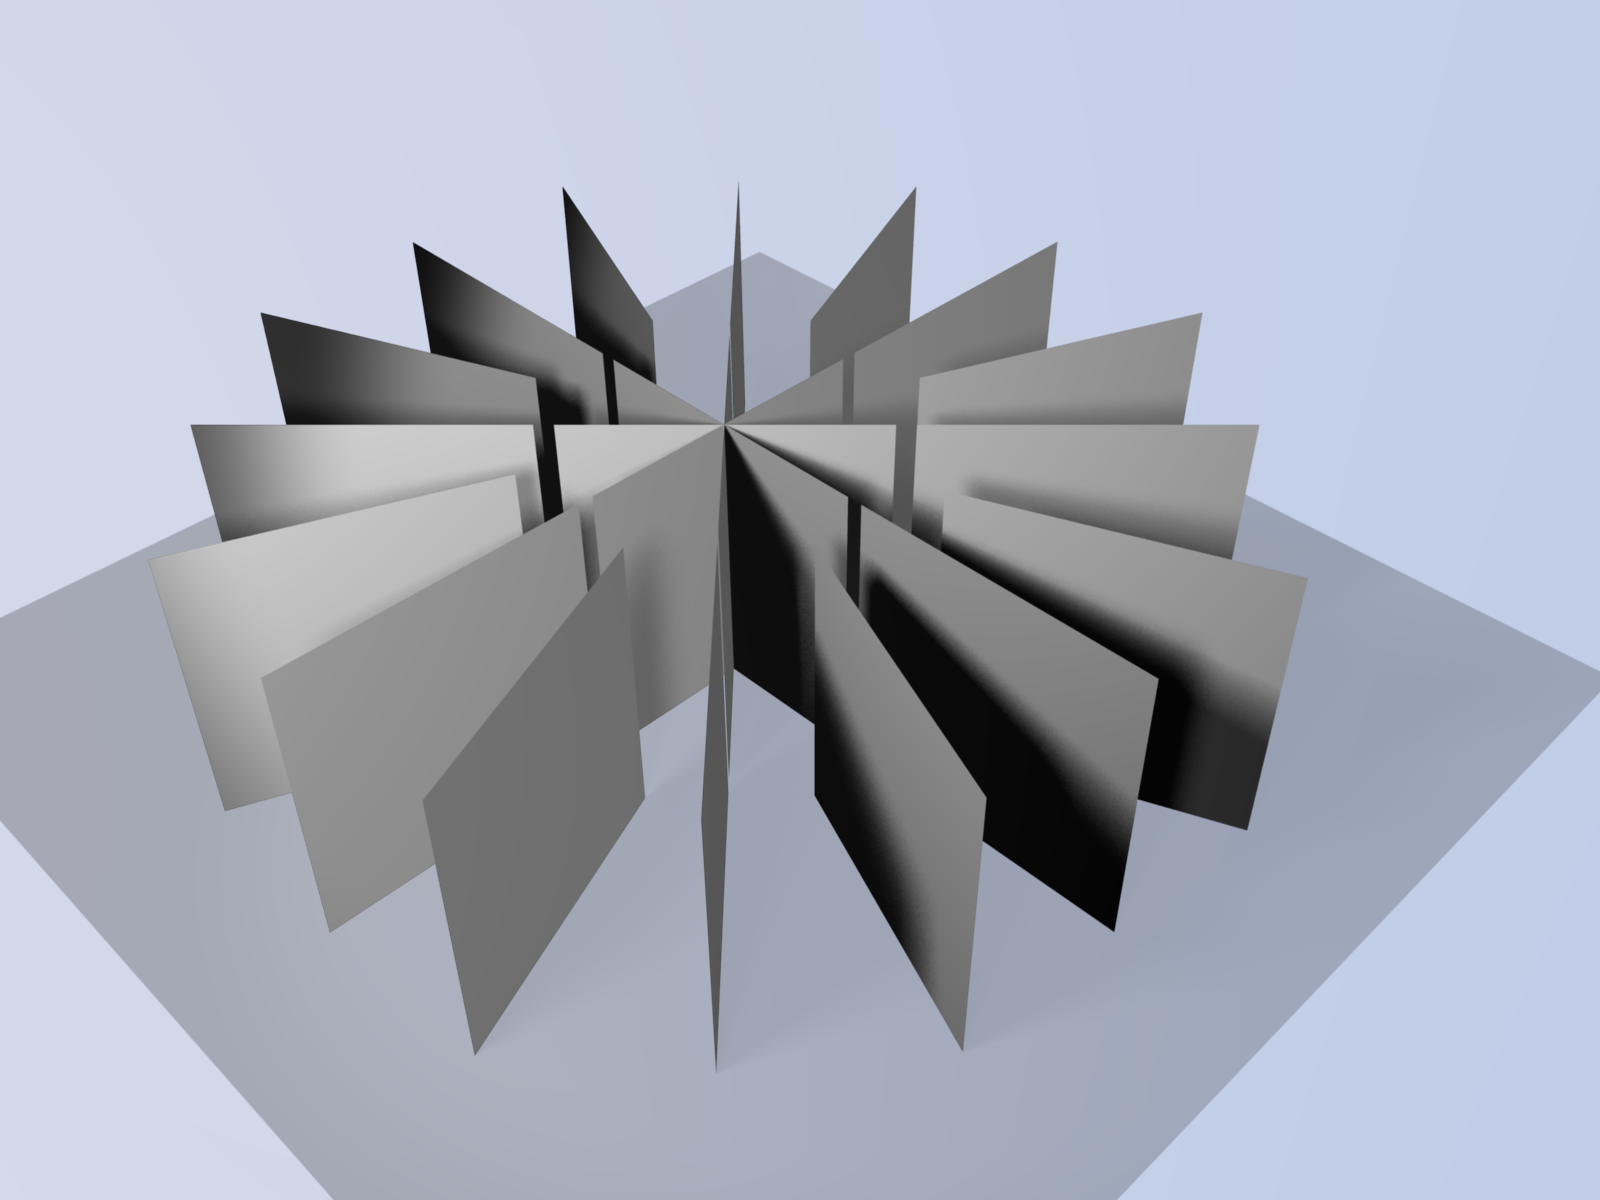
\includegraphics[width=\imsize]{img/projections}
	\caption{Projection Setup with one central and one ring-scan}
	\label{fig:projections}
\end{figure}